For this study, an experiment was implemented using the \emph{roborobo} simulator\cite{bredeche_roborobo!_2013}.
Even though \emph{roborobo} contains some functionality for running robot simulations, a lot of modifications were needed for the simulator to fit the needs of this experiment.
This chapter will include a description of \emph{roborobo}, the modifications that were made to the existing software, the experiment in general and the motivation for its implementation.

\section{Experiment motivation}
The introduction lists several research questions that this project is aiming to contribute.
To not trivialise the environment and the interaction between the robots, care was taken when designing this experiment.
The thought behind the experiment is to see collective behaviour using an evolutionary algorithm.
Caution was taken to implement an unbiased system in regards to the influence it imposes on the algorithm to achieve correct and analyzable results.  
For example, the evaluation function in section \ref{sec:evaluation} is quite simple and does not add any guiding parameters to promote self-assembly.

One of the questions concerns how collective decision-making influences the emergence of self-assembly.
Swarm behaviour found in nature displays how simple agents collectively can make a decision.
The goal of this experiment is, therefore, to design a similar environment to promote this form of collective behaviour.
In this environment, the robots have to form swarms for survival, and collectively decide if they should self-assemble or attempt an escape.

By design, the robots are given a local communication module that can be used to send an array of floating point numbers to its neighbours in the self-assembly structure\ref{sec:local_comm}.
The influence of the communication module and the values that the communication packets take are entirely governed by the neural network \ref{sec:ctrnn}.

The system has also been made to be highly configurable such as many of the evolutionary algorithm parameters as well as general environmental setup. 
By varying the parameters of the experiment, it is possible to observe and analyse the problem statements which were discussed in chapter \ref{ch:introduction}.
Depending on the configuration used when running the simulation, it should be possible to see how different assembly protocols and behaviours emerge, and how the self-assembly behaviour of the robots differ from similar trials and different configurations.
Chapter \ref{ch:results_and_discussion} portrays the results and analysis of this experiment.


\section{Experiment setup}
\label{sec:description}
For this experiment a micro-organism environment is imagined, where the organisms find themselves in some liquid pool. 
The micro-organisms are the agents in our system and are represented as swarm bots.
The main functions of the robots are, in addition to movement, foraging and self-assembly.

The robots find themselves in a pond.
In the pond there are nutrients which the robots can feed on to replenish their energy.
At the same time the pond also contains larger predator organisms which wants to feed on the robots.
It is imagined that the robots can assemble to form larger structures.
The robots can protect themselves from the predator organisms by forming a larger structure which the predator is unable to eat.
When the robots are assembled they may eat the larger predator to replenish energy as well.
The predators come in multiple sizes, and to gain an advantage the robots must form a large enough structure.
Maintaining the assembled structure cost energy, and the robots therefore have an incentive to disassemble once the structure is no longer required.

\section{Environment}
The imagined pond environment can be represented as a rectangular box(figure \ref{fig:environment}), containing the robots, nutrients and predators.
Initially, the environment is populated with nutrients, robots, and predators placed at random positions in the environment.
When a nutrient is consumed, a new one is placed at a random position in the environment.

\begin{figure}[H]
	
	\centering
	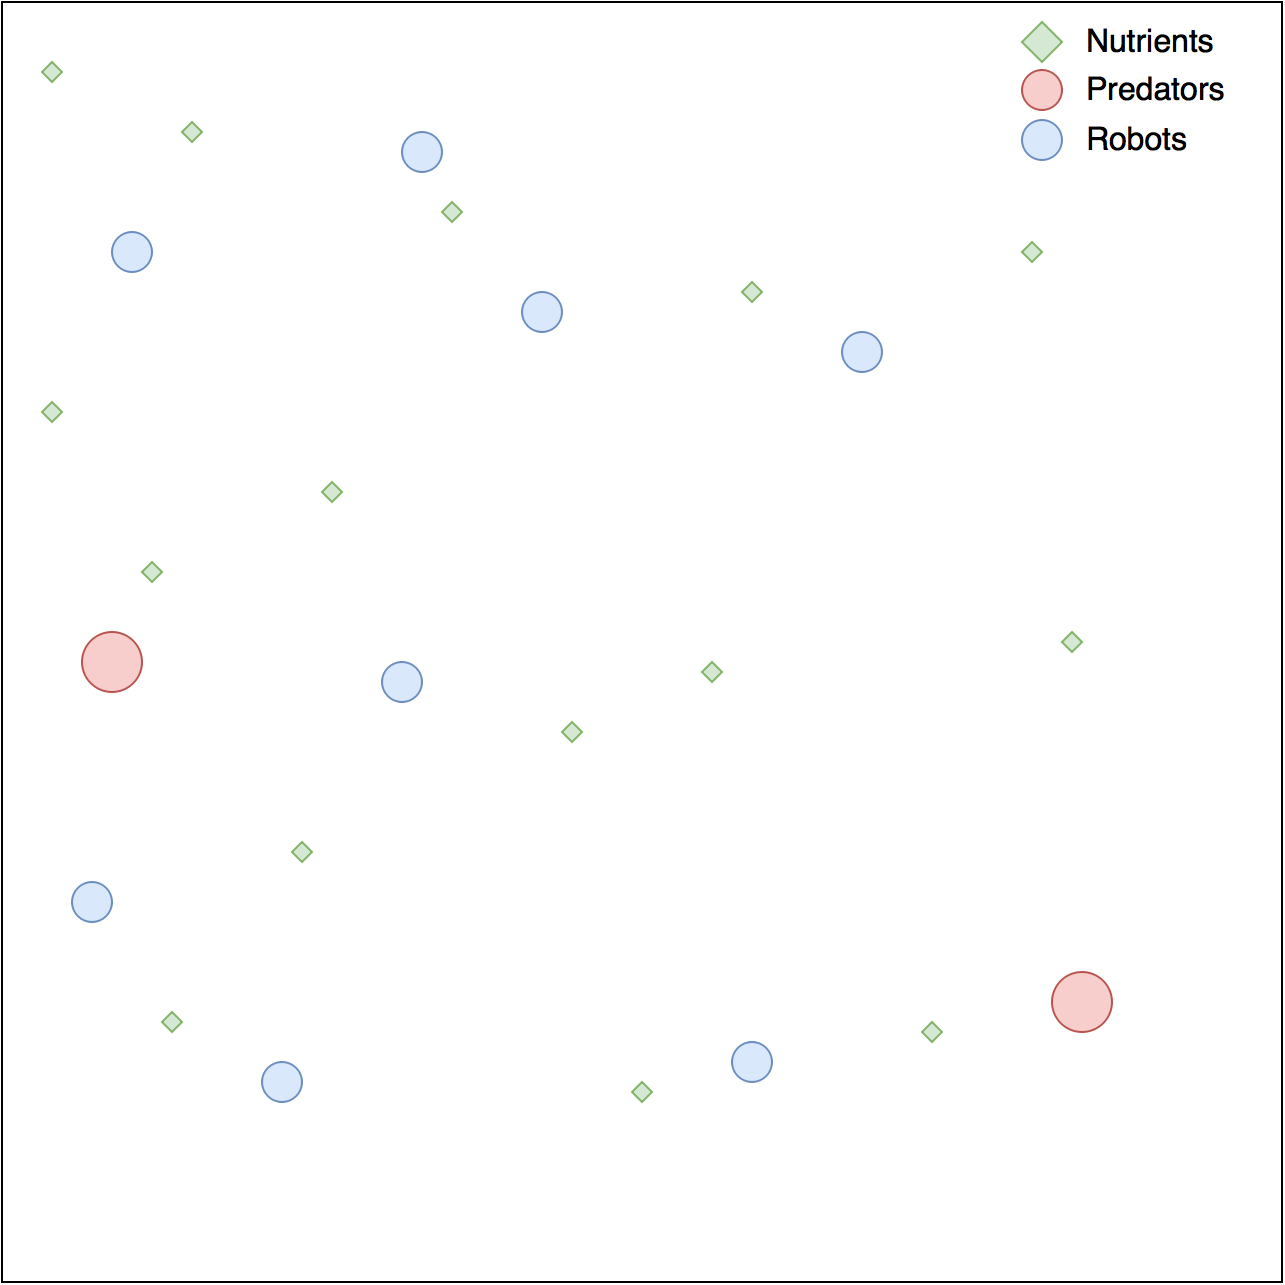
\includegraphics[width=0.65\textwidth]{chapters/res/Environment.png}
	\caption{Initial configuration of the environment.}
	\label{fig:environment}
\end{figure}


\section{Roborobo overview}
The programming interface for roborobo is divided into three components(\emph{World observer, Agent observers, Agent controllers})\cite{bredeche_roborobo!_2013}.
Each robot in the simulation receives an instance of the \emph{agent controller} and the \emph{agent observer}.
The philosophy of the roborobo framework is that the programmer should implement the robot behaviour in the \emph{agent controller}, and use the \emph{agent observer} and \emph{world observer} to access state about agents and the world.
This relationship is visualised in figure \ref{fig:component-relationship}.

\begin{figure}[H]
	\centering
	\begin{subfigure}{0.31\textwidth}
		\label{fig:controller}
		\centering
		\hspace*{1.15cm}\includegraphics[height=\linewidth]{chapters/res/agent_controller.png}
		\caption{}
	\end{subfigure}
	\begin{subfigure}{0.31\textwidth}
		\label{fig:agent-observer}
		\centering
		\includegraphics[height=\linewidth]{chapters/res/agent_observer.png}
		\caption{}
	\end{subfigure}
	\begin{subfigure}{0.31\textwidth}
		\label{fig:world-observer}
		\centering
		\includegraphics[height=\linewidth]{chapters/res/world_observer.png}
		\caption{}
	\end{subfigure}
	\caption{The relationship between a) the agent controller, b) the agent observer, and c) the world observer. }
	\label{fig:component-relationship}
\end{figure}

Each robot in the simulation also receives a component called a \emph{world model}.
The world model contains an agent specific representation of the outside world.
The model includes states such as sensors readings and current velocity.

The observers can be used to perform tasks that are not directly related to the robot behaviour.
In each simulation step the observers are run before any of the \emph{agent controllers} are run.
This means that the observers have a stable snapshot of the world between each update.
The observers are therefore useful for performing tasks that should be carried out between each update of the world.
Examples of useful applications of the observers are updating the agent's world models, monitoring, logging, computing fitness, and managing evolutionary algorithms.
In the standard case, understanding the components described in this section is sufficient to perform a wide variety of simulations.

The depicted experiment in this chapter is not realizable with the basic roborobo framework.
The necessary modifications to the framework are described in section \ref{sec:modifications}.

\section{Roborobo modifications}
\label{sec:modifications}
As mentioned in the description, roborobo does not support self-assembly out of the box.
Self-assembly support, therefore, requires adding additional abstractions to roborobo.
This section includes the different modifications that were made to the roborobo framework to support self-assembly, local communication, and a configurable system.

\subsection{Robot Groups}
The high-level abstraction that encapsulates the behaviour for connected robots is called a \emph{Robot group}.
All robots that are capable of self-assembly are robot groups.
Single robots that are not connected are simply robot groups with one member.
The responsibilities of the robot group are to take care of group movement, handling collisions, connecting and disconnecting. 
	
\subsubsection{Movement}
In the roborobo framework, the robots movement is decided by the robot controller by requesting a certain angular and translational velocity.
The movement of a group is decided by first converting the desired direction and velocity into a translation vector.

\begin{equation}
\centering
\vec{v_{xy}} = v\cdot[\cos(\theta), sin(\theta)]
\end{equation}

The combined movement of the group is then decided by averaging the translation vectors from each member in the group.

\begin{equation}
\centering
\vec{v_t} = \frac{1}{n}\sum_{i=0}^{n} \vec{v_{i}}
\end{equation}

Once the translation vector for the group is computed, it can be applied to each member of the group by converting it back to the format of direction and velocity that roborobo uses.

\subsubsection{Collisions}
Roborobo already performs collision detection for robots, but in robot groups, some additional logic is required.
The collision behaviour for robots is that if they collide with a solid object, they stop.
This behaviour is a problem for groups of more than one robot because if one robot collides it may get left behind by the rest of the group.
This issue is solved by backing up the position of each robot in a group before applying the computed translation.
If a robot in the group collides with something, the robots in the group are reverted to their original position

\subsubsection{Connections}
The connections between robots in a group can be considered a graph, where the robots are nodes and connections are edges.
Connecting robots can then be treated as simply adding an edge between the two nodes representing the robots.
Similar to connecting, disconnecting consists of removing the edge between the nodes representing the robots.
In the case that a robot has multiple connections in the group extra care has to be taken because removing one edge may split the graph into two smaller sub-graphs.
If this occurs, the two sub-graphs must now be treated as two new separate groups.
It can be determined if a robot can simply be disconnected, or if we have to split the group by finding out if there is a cycle that leads back to the robot that is to be disconnected.
The existence of a cycle is determined by first removing the edge representing the connection, and then performing a depth first search.
	 
\subsection{Docking mechanism}
As described in section \ref{sec:mechanisms}, there is a wide variety of docking mechanisms used in earlier projects.
The docking mechanism implemented is therefore highly configurable, to support a wide variety of different mechanisms.
The configurable properties are as following, the number of ports, the placement of ports, and different genders for the ports. 

\subsubsection{Connection validation}
The robots can attempt a connection at any time; this requires a procedure to make sure the attempted connections are valid.
Three requirements have to be met before a connection can be established between robots.
First, the ports have to be spatially sound. 
Here, the distance between the ports has to be less than a threshold value.

\begin{equation}
|\vec{p_1} - \vec{p_2}| < \epsilon
\end{equation}

Next, the position of the ports has to be geometrically sound.
Here, the angle between the connection ports has to fit within a threshold range.

\begin{equation}
180 - \epsilon < |\theta_1 - \theta_2| < 180 + \epsilon
\end{equation}

Finally, the gender of the ports must be compatible, meaning one of them is female while the other is male or at least one of the connection ports being universal.
		
\subsection{Local communication}
\label{sec:local_comm}
The robots are equipped with a communication module that allows local communication with their connected neighbours.
The message format is very simple; the robots can only broadcast "packets" of floating point numbers.
The size of the packets is equal to the number of connection ports.
At the receiving end, the packets sent by neighbours are aggregated into a single packet.
The aggregation is performed by adding the components of each message packet with the corresponding components from the other message packets. Figure \ref{fig:local_communication} illustrates this process.

\begin{figure}[H]
	\centering
	\includegraphics[width=0.65\textwidth]{chapters/res/Local_communication.png}
	\caption{Robot B aggregating the messages received from robot A, and C.}
	\label{fig:local_communication}
\end{figure}

In the robot controller, the messages from the communication module are fed into dedicated message input neurons, and the value of the message output neurons are broadcast to the neighbours.

		
\subsection{Predators}
A crucial part of the environment in the simulation are the predator robots.
These robots are not under the influence of the evolutionary algorithm and rather uses a much simpler pre-programmed controller.
The predator robots have two basic actions that can affect the system: the predators can either eat prey or explore the envelopment.

\begin{figure}[H]
	\centering
	\frame{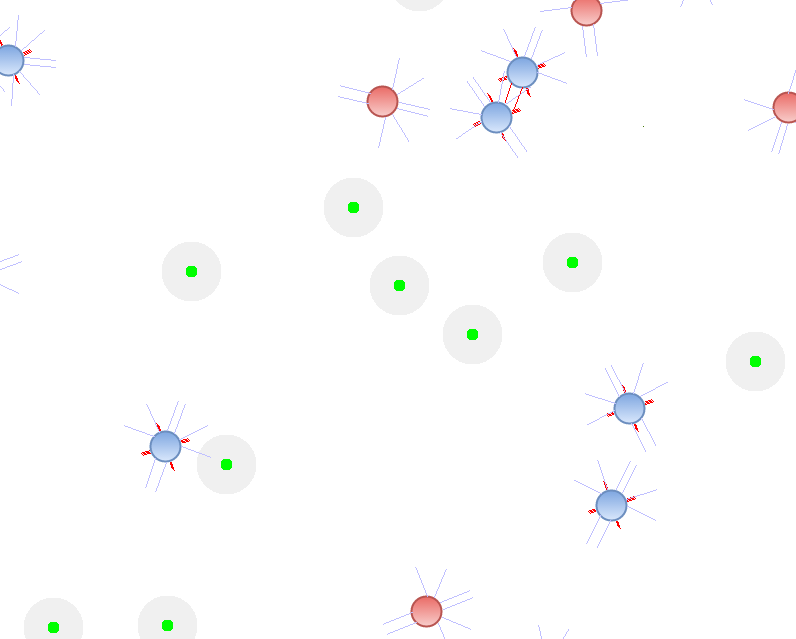
\includegraphics[width=0.65\textwidth]{chapters/res/predator_snippet.png}}
	\caption{A screenshot of a simulation. The predators are marked with red and the robots guided by the evolutionary algorithm are marked with blue}
	\label{fig:predator_screendump}
\end{figure}

As seen in figure \ref{fig:predator_screendump}, the predators also uses six sensors which they use to decide if they are colliding with an object and what that object is.    
Concerning exploration, the predator controller uses a simple object avoidance tactic.
If the predator robots sense an object on any of its side sensors, it will change its rotational velocity to avoid this object.
In practice, this means that if the predator senses an object on the right, it will steer left, and vice versa.
A slight random rotational velocity is added such that its movement becomes more dynamic in the case where there is no collision.
This object avoidance behaviour is always employed as long as it does not sense a robot(prey).
In this case, it will have the opposite behaviour and turn towards the object, as it intends to consume the prey.

In addition to movement, the predators can also consume a robot. 
Predators consume a robot when there is a collision between a normal robot and a predator robot.
If a robot is consumed, it is removed from the environment and robot's lifetime is recorded for use in the fitness function of the evolutionary algorithm. 
For a predator to be able to eat a robot, the robot must not be part of a robot group of a size less than some configurable threshold.
The default threshold is set to three for the simulations run in this experiment.
The reason for this is to give the regular robots some advantage of self-assembling in hopes of potentially evolving this behaviour. 

\subsection{Energy drain}
In addition to the environmental hazards of predators, the robots also must face the issue with having a limited energy supply.
If a robot loses all if its energy, then it will die and be removed from the environment.
Five main configurations handle the energy parameters of the simulation:

\begin{itemize}
	
	\item \emph{gEnergyMax}, is a constant which represents the maximum amount of energy the robot can hold.
	If a robot picks up more energy from an energy source and the total energy exceeded \emph{gEnergyMax}, then the total energy will simply be \emph{gEnergyMax}.
	
	\item \emph{gEnergyInit}, is a configurable parameter which sets the initial energy of a robot when spawned into the environment.
	
	\item \emph{gEnergyItemDefaultInit}, is the store of energy an energy item in the environment holds.
	
	\item \emph{gPassiveEnergyDrain}, is the leak value of energy of a single robot. At each time step, a robot loses \emph{gPassiveEnergyDrain} amount of energy.
	
	\item The final energy parameters is \emph{gConnectionEnergyDrain}, which is an addition drain for being self-assembling with another robot.
	
	
\end{itemize}


The reason for adding an energy hazard for the robots in this experiment is to give them a non-trivial self-assembling scenario.
If predators were the only environmental obstacle, then the robots would most likely develop a self-assembly strategy and hold this construction in remaining time of simulation.
It is intended that the robots would have an environment which allowed strategies such as dissembling the self-assembly structure to evolve or perhaps not even self-assemble at all.
This reasoning is also the justification for giving the robots additional energy drain when assembled

\section{CTRNN}
\label{sec:ctrnn}
For this project, an artificial neural network that has gained a lot a popularity in regards to robotics known as Continuous-Time Recurrent Neural Network (CTRNN) was implemented. 
The CTRNN was researched and developed by Randall Beer\cite{beer_dynamics_1997} and adds two new properties to the standard artificial neural network. 
The properties that are introduced in CTRNN is a time constant and a gain constant.

As most neural networks, the simple integration of the inputs from all neighbouring neurons are added giving us the first standard equation for neural networks:

\begin{equation}
s_i = \sum_{j=1}^{n}o_{j}w_{i,j}+I_i
\end{equation}
\\
Here, $o_j$ represents the output(after activation) of neuron $j$, $w_{i,j}$ is the weight from neuron $j$ to neuron $i$ and $I_i$ is the sum of all the external inputs to node $i$.

\begin{equation}
\frac{dy_i}{dt} = \frac{1}{\tau_i}[-y_i + s_i + \theta_i]
\end{equation}
\\
In order to preserve the previous state of the ANN, the internal state is stored. 
$y_i$ denotes the internal state of neuron $i$.
To derive the next internal state, Beer computes $\frac{dy_i}{dt}$ as a combination of the following inputs and the current internal state of the node, where a time constant $\tau_i$ decides the rate of drain. 
$\theta_i$ is a term added for a neuron-specific bias.
It is only added here for mathematical soundness as it is simply added as a bias node during implementation and hence incorporated in $s_i$.
The time constant $\tau_i$ is what gives CTRNNs the ability to produce rich functionality and convincingly sophisticated cognition.
If $\tau_i$ has a low value, then we will have a high degree of drain and hence having its new input dominate the next state.
However, if $\tau_i$ has a high value, then we have a higher degree of memory because its previous state will dominate the next state.

\begin{equation}
o_i = \frac{1}{1 + e^{-g_{i}y_{i}}}
\end{equation}
\\
To convert the internal state to an output $o_i$, Beer typically uses sigmoidal activation function.
A sigmoidal activation function is typical in other neural networks as well, but Beer also employs a gain term $g_i$, to influence the activation of the neuron.
\\
\begin{figure}[H]
	\centering
	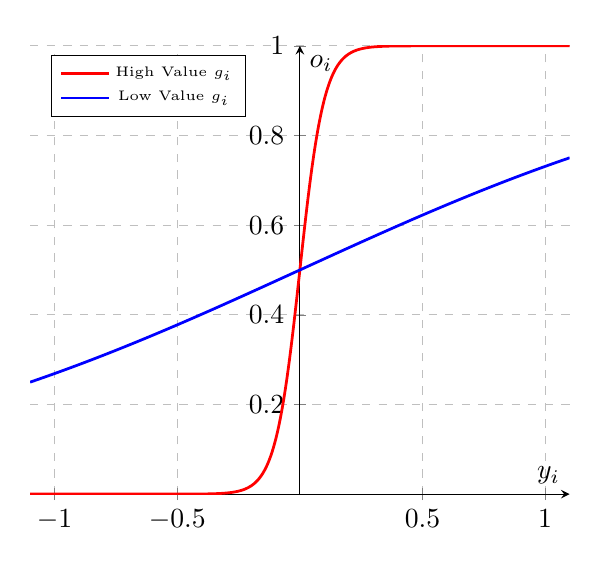
\begin{tikzpicture}
	\begin{axis}[
	axis lines = center,
	xlabel = $y_i$,
	ylabel = {$o_i$},
	ymajorgrids=true,
	xmajorgrids=true,
	grid style=dashed,
	legend style={at={(0.22, 0.98)},anchor=north, font=\tiny}
	]
	%Below the red parabola is defined
	\addplot [
	domain=-1.1:1.1, 
	samples=500, 
	color=red,
	line width=1pt,
	]
	{1/(1+e^(-20*x)};
	\addlegendentry{High Value $g_i$}
	%Here the blue parabloa is defined
	\addplot [
	domain=-1.1:1.1, 
	samples=100, 
	color=blue,
	line width=1pt,
	]
	{1/(1+e^(-1*x)};
	\addlegendentry{Low Value $g_i$}
	
	\end{axis}
	\end{tikzpicture}
	\caption{The difference in the activation function with respect to $y_i$ based on a low and high value of $g_i$}
	\label{CTRNN-gGraph}
\end{figure}

As seen in figure \ref{CTRNN-gGraph}, the value of the gain parameter can influence the activation function in such a way that it can be a smooth, almost linear, function or it can take on the behaviour of an activation function resembling a switch.
Having the ability to change the activation function on a neuron to neuron basis, is the second reason(the first being time constants) CTRNNs can give rise to complex and rich behaviour.


\subsection{Topologies}
%Sensors(6), connection status(n), messages(n), 1 energy level.
In the robot controller, the neural network is responsible for making decisions.
The role of the robot controller is to forward inputs to the input layer of the neural network and interpret the output.
The information that the neural network is provided with is as follows: sensor readings, the connection status of each docking port, messages from the communication module, and finally the current energy level of the robot.
Once the inputs are processed the robot controller reads the output layer to decide the values for the motor functions, control of the connection ports, and the message to be sent via the communication module.
The number of hidden layers and the number of neurons in each of them is configurable at runtime.

The robots have to be able to detect, and distinguish between predators, other robots, food, and the environment.
The robots are equipped with six sensors to achieve this.
To represent this two different input topologies for the sensors have been implemented.

\subsubsection{Dense}
The dense topology uses 24 nodes to represent the inputs where there is one node per sensor for each of the four different objects that can be detected.
With this configuration, the robot can distinguish between multiple types of objects at the same time.
The motivation for designing another input topology is the concern that by using 24 nodes the search space for the evolutionary algorithm may become too large to find a good solution within a reasonable time.

\subsubsection{Sparse}
The sparse topology is a compromise between the number of nodes and the robots ability to distinguish between multiple objects at the same time.
Here the input layer has six nodes for each of the sensors, and four additional nodes that indicate whether a particular type of object is currently detected by one of the sensors.
This modification brings the number of input nodes for the sensors down to 10, instead of 24.
With this configuration, the robot can still detect nearby robots, but it can not differentiate between multiple types of objects at the same time.

			
\section{Evolutionary algorithm}
The following section describes the implementation of the evolutionary algorithm for this project.
In addition, in some of the sections, multiple implementations are mentioned.
We see an occurrence of this in section \ref{mutation_operators} where both random and incremental mutation operators being explained.
The reason multiple implementations were done is due to the initial implementation yielding poor results and hence there was made an attempt at improving the results.

\subsection{Genotype}
\label{sec:genotype}
The genotype contains the weights, gains and time constants for the neural network used in the robot controller.
During run-time, the genotype size is fixed and depends on the size of the neural network.
The size of the neural network is configurable (topology and size of each layer) in the simulation configuration file, and hence, the genotype can change size depending on the simulation run.
The structure of the genotype is an array of double precision floating point numbers in the range $(-1, 1)$.
Each number in the genotype represents a specific weight, gain, or time constant in the neural network.
Before the genotype can be used to configure the neural network the values are mapped into the suitable range for each type of parameter, figure \ref{fig:genotype-mapping}.
The selected range, $(-1, 1)$ used for the values in the genotype is, therefore, arbitrary, and holds no particular significance. 

\begin{figure}[H]        
	\centering
	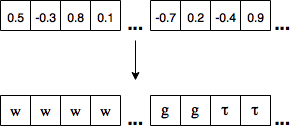
\includegraphics[width=0.80\textwidth, clip]{chapters/res/genotype_translation.png}
	\caption{Mapping the genotype into weights, gains, and time constants.}
	\label{fig:genotype-mapping}
\end{figure}

\subsection{Initialization}
As seen in theory, there are two ways to initialize a population. 
It can be done completely random, or there can be a more particular initialization with bias. 
In the case of this experiment, a purely random initialization was implemented.
The reason for this is that there is no trivial functionality that these robots should have for it to reach the most optimal solution.

Since this experiment is about researching self-assembly, one might think that initializing our robots with a behaviour to promote this, could be beneficial.
There are two main issues with an approach like this.
First, self-assembly in this complex system is an emergent behaviour(see ch. \ref{sec:complex_systems}).
This means that there is no trivial configuration of the neural network that gives rise to self-assembly.
It is rather, emergent from the robots' behaviour and their connections with each other in the environment.
As explained in chapter \ref{ch:background}, there are mechanisms such as the assembly protocol, the assembly architecture, and also the hardware mechanisms used.
None of these mechanisms can simply be coded into a neural network.

The second issue with implementing a bias towards self-assembly is that this might not be the best survival strategy in this experiment.
Even though the experiment is designed to give the robots a slight benefit from self-assembling, this might not be the case in reality.
Due to these two reasons, it was decided to have a strictly random initialization.

\subsection{Mutation operators}
\label{mutation_operators}
As seen in section \ref{sec:evo_alg}, the proper step after mating genotypes is applying a mutation to the resulting genome.
Mutation is done using a mutation operator.
During the implementation of the experiment, two different mutation operators were implemented, the random mutation operator and the incremental mutation operator.

During the first iteration of implementation, a standard random mutation operator was implemented.
As explained in \ref{sec:genotype}, the genotype is modelled using doubles, so a random mutation operator for this implementation simply re-rolls the selected double, $x$, to a new double where $x \in [-1.0, 1.0]$. 
The number of weights to be mutated is configurable and is represented as some percentage, \emph{mutation rate}.

\subsubsection{Incremental}
During initial trials, it was observed that the impact of completely changing the value of a weight in the neural network could potentially drastically change the behaviour of the robots.
The change in behaviour yielded poor results of the evolutionary algorithm because of constant destabilisation of the emergent behaviours.
The results from the preliminary trials caused an incremental mutation operator to be implemented.
The incremental mutation operator gave better results than the random mutation operator, so it was decided that the random mutation operator should be removed from the system. 
The incremental mutation operator works in a similar manner as the random operator, where a weight is chosen for mutation at some percentage, but instead of completely re-rolling its value, it only differs from its original value by a certain threshold.
The incremental mutation still causes a mutation to occur, but it will not be as drastic, yielding smoother results. 

\begin{figure}[H]
	\centering
	\begin{subfigure}{0.3\textwidth}
		\label{fig:mutation-random}
		\centering
		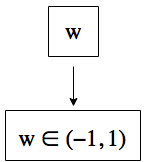
\includegraphics[height=\linewidth]{chapters/res/mutation_random.png}
		\caption{}
	\end{subfigure}
	\begin{subfigure}{0.3\textwidth}
		\label{fig:mutation-incremental}
		\centering
		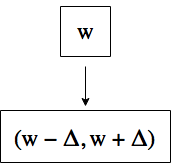
\includegraphics[height=\linewidth]{chapters/res/mutation_incremental.png}
		\caption{}
	\end{subfigure}
	\caption{ }
	\label{fig:mutation-operators}
\end{figure}

\subsection{Selection mechanism}
The selection step of an evolutionary algorithm is responsible for selecting which individuals should become parents.
In other words, it applies selection pressure.
If the selection pressure is too high, the algorithm may converge prematurely, and if it is too low, the search may take more time than necessary.
For the experiment, two different selection mechanisms have been implemented.

The first selection scheme that was implemented in this project was \emph{proportional selection}.
In this selection scheme individuals are selected for reproduction with a probability proportional to their fitness compared to the total fitness of the population.
It is common to apply a scaling function on the fitness in the population to adjust selection pressure.
A scaling function that is often used with proportional selection is \emph{Sigma scaling}\cite{goh_sexual_2003}, which was also initially used in this experiment:

\begin{equation}
S(f, \overline{f}, \sigma, s) = s + \frac{f - \overline{f} }{2\sigma}
\end{equation}

where \emph{f} is the fitness of an individual, $\overline{f}$ is the mean fitness of the generation, $\sigma$ is the fitness variance, and \emph{s} is a scaling factor that can be used to adjust the selection pressure.

Sigma scaling modifies the selection pressure introduced in the raw fitness by using the populations fitness variance as a scaling factor.
The scaling has the effect of dampening the selection pressure when there are a few individuals with an exceedingly higher fitness than the rest and increasing the selection pressure when the population has a low variance.

The values obtained from the scaling can now be used to select parents by sampling the distribution.
\emph{Roulette wheel selection}(RWS)\cite{goh_sexual_2003}  is one such method.
RWS can be visualized as giving each potential parent a sector with size relative to the scaled fitness in the roulette wheel(figure \ref{fig:roulette}).
The parents are then selected by spinning the wheel until the desired number of parents are picked.

\begin{figure}[H]
	\centering
	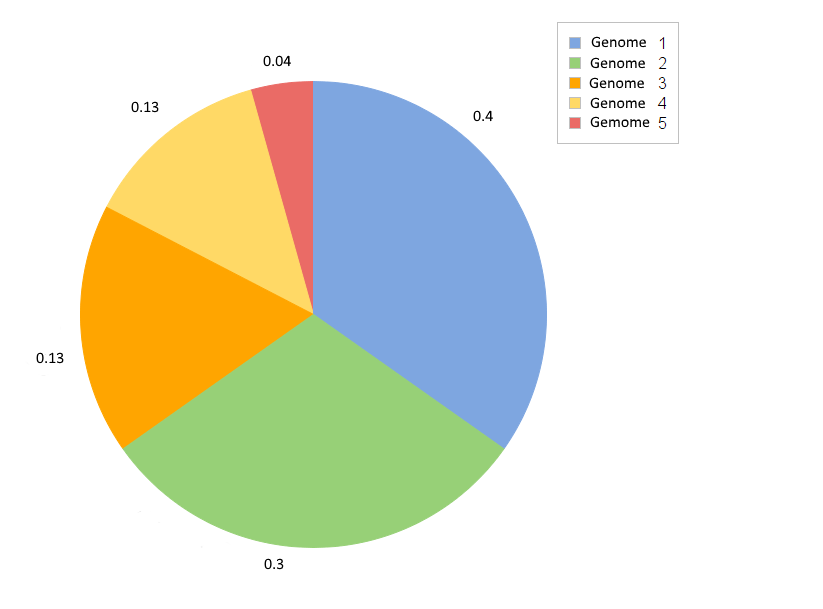
\includegraphics[width=0.80\textwidth, clip]{chapters/res/roulette.png}
	\caption{A roulette wheel where the size of each sector represents the probability of picking a particular parent.}
	\label{fig:roulette}
\end{figure}

The roulette wheel implementation gave less compelling results than expected, which caused tournament selection to be implemented which gave better results and caused the roulette wheel selection mechanism to be removed from the system.		
\subsubsection{Tournament selection}
In contrast to proportional selection the individuals do not compete with the entire population but instead, compete within groups selected at random.
Tournament selection performs parent selection by picking individuals at random into a group.
From the group the fittest individual is selected as the parent.
This process is repeated until the desired number of parents have been selected.
The group size varies between implementations, but typical implementations compare two\cite{goh_sexual_2003} individuals at a time, depicted in figure \ref{fig:tournament}

\begin{figure}[H]    
	\centering
	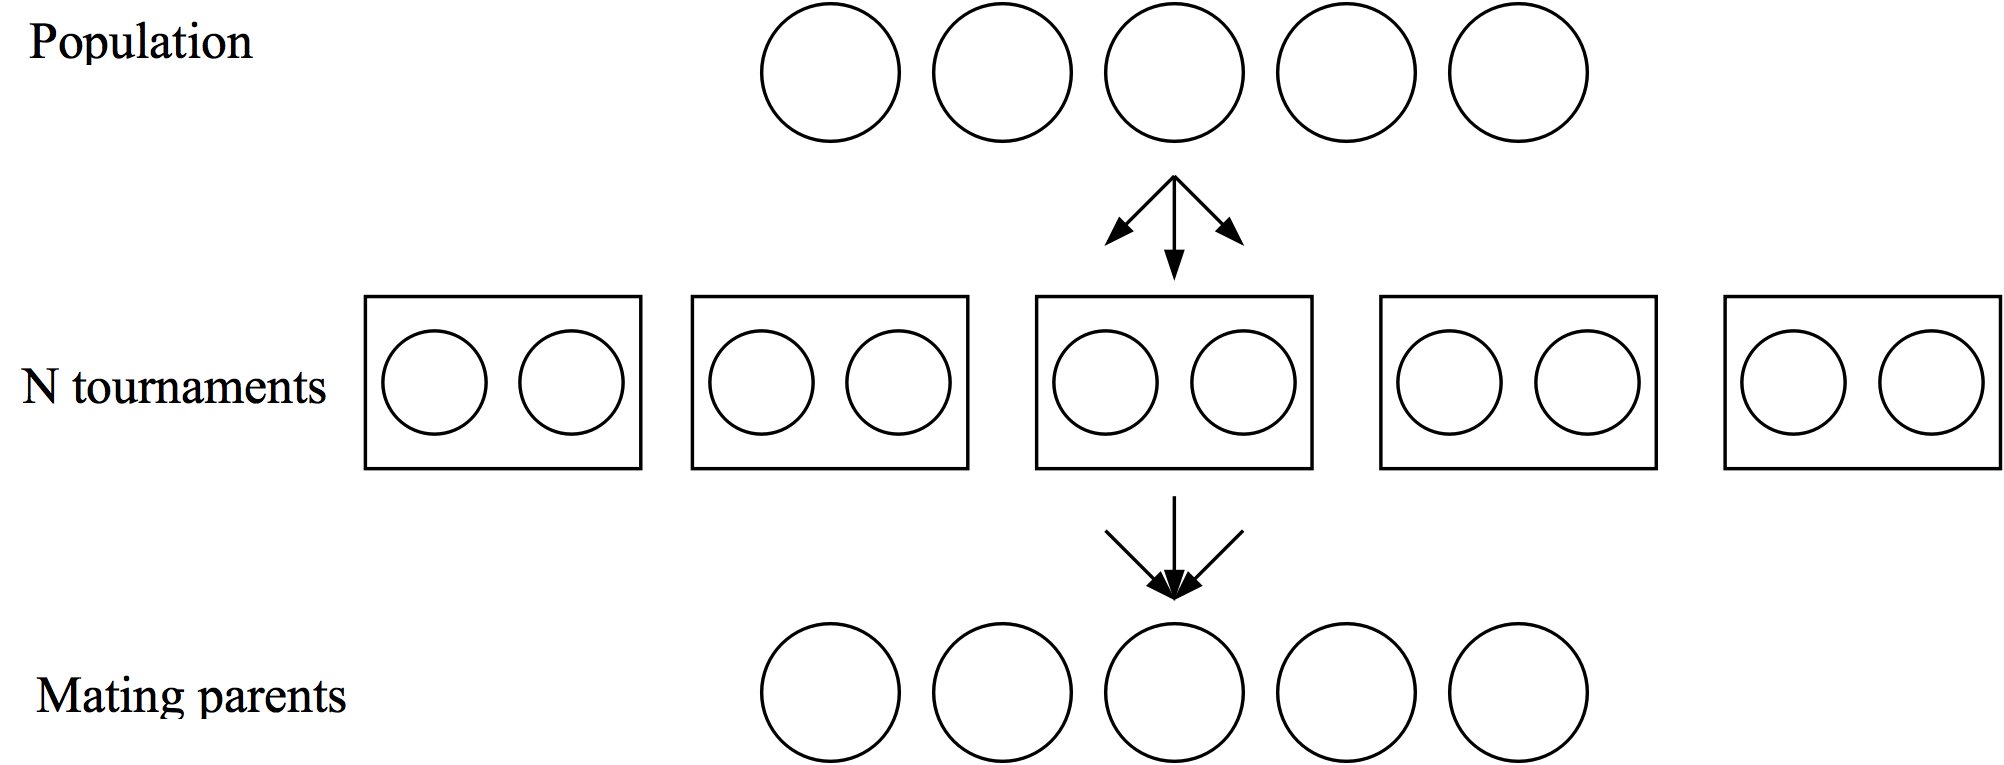
\includegraphics[width=\textwidth, clip]{chapters/res/Tournament.png}
	\caption{Selecting parents using a binary tournament.}
	\label{fig:tournament}
\end{figure}

The described process introduces a high selection pressure since it selects the fittest individual from each group.
It is common to include an acceptance threshold, $t$, into the selection to modify the selection pressure\cite{goh_sexual_2003}.
Each time an individual is to be selected a random number $r \in (0, 1)$, is generated.
If $r < t$, then the fittest individual is chosen. 
Otherwise, the less fit individual is chosen. 
The selection pressure can then be tuned by increasing or decreasing the acceptance threshold. 
A lower value for $t$ decreases the selection pressure, while a higher value increases the selection pressure.

\subsection{Elitism}
In each step of the evolutionary algorithm, the previous generation is replaced by the offspring of the selected parents.
Completely replacing the previous generation with the new generation has the undesirable effect where mutations in the children can lead to the loss of good partial solutions.
A configurable level of elitism has therefore been implemented into the evolutionary algorithm.
At the end of each generation, the $n$ fittest individuals are promoted to \emph{elites}, who are then allowed entry into the next parent selection unchanged.
Elitism allows multiple generations to build upon the partial solutions in the elites and ensures that the fittest genomes are preserved between generations.

\subsection{Evaluation}
\label{sec:evaluation}
The evaluation function was kept fairly simple as to restrain from guiding the robots.
Primarily, the evaluation function was only calculating how many robots survived the trial.

\begin{equation}
\label{eq:basic_fitness}
f(G) = \frac{G(\bar{R_{tot}})}{R_{tot}}
\end{equation}

where $f$ is the fitness score of some genome $G$.
$G(\bar{R_tot})$ is the number of robots that died, $\bar{R_tot}$, in the trial with genome $G$, and $R_n$ is the total number of robots in the system.

This fitness function, however, gave poor results mainly due to the fitness graph being discrete and failing to differentiate enough between different genomes.
Therefore, a different approach was implemented where the lifetime of a robot used instead.

\begin{equation}
f(G) = \frac{\sum_{i=1}^n G(L_i)}{nL_{max}}
\end{equation}

The fitness of a genome is calculated in a similar way as eq. \ref{eq:basic_fitness}.
The difference here is is that $L_i$ represents the lifetime of robot $i$ during simulation, $n$ is the total number of robots, and $L_{max}$ is the maximum lifetime of a robot.
It is also possible to add addition fitness for the ability to aggregate such that self-assembly(or at least proximity) is promoted, but as mentioned earlier, the purpose was to limit the amount of evolutionary guiding.
In the case where self-assembly does not occur, a more sophisticated objective function could be implemented.
		
\clearpage
\section{Data gathering}
The statistics logged for post-processing, and later analysis is as follows:
\begin{itemize}
	\item Fitness
	\item Group size
	\item Number of groups
	\item Food collected by individual robots
	\item Food collected by robot groups
	\item Number of predators eaten by robot groups
	\item Number of robots starved
	\item Number of robots eaten by predators
\end{itemize}
These statistics are logged at the end of each scenario for every genome in all the generations.
These statistics are recorded by the agent observers and the world observer, the only exception being energy collected which required some additional modification of roborobo.
Which consisted of performing the logging when energy is rewarded for eating food.
Logging the group sizes, and the number of groups is done a bit differently than the rest of the statistics.
The logging is performed by taking a snapshot which contains the number of groups and their sizes every 50 iterations of the simulation.
The reason for this is that they change in value over the lifetime of a simulation, and this change should be recorded.



\clearpage
